\documentclass[11pt,spanish,letter]{article}

\usepackage{graphicx}
\usepackage{rotating}
\usepackage{rotfloat}

\DeclareGraphicsExtensions{.pdf,.eps,.svg}

\usepackage[spanish]{babel}
\usepackage[utf8]{inputenc} 

\usepackage{fancyhdr}
\usepackage{vmargin}
\usepackage{varioref}
\usepackage{hyperref} 
\usepackage{xspace}
\usepackage{float} 
\usepackage{subfigure}
\usepackage{latexsym}
\usepackage{amsmath}
\usepackage{amsfonts}
\usepackage{amssymb}
\usepackage{relsize}
\usepackage{tabulary}
\usepackage{alltt}	% required for `\alltt' (yatex added)

\usepackage{url}
\usepackage{listings}

\usepackage [boxed, ruled, lined, vlined, linesnumbered]{algorithm2e}

\newcommand{\refe}[1]{\S~\ref{#1}\xspace}

\newcommand{\producer}{\operatorname{Prod}}
\newcommand{\owner}{\operatorname{Prop}}
\newcommand{\good}{\operatorname{B}}
\newcommand{\process}{\operatorname{Proc}}

\newcommand{\bigo}{\mathcal{O}}

\newcommand{\bien}[1]{\mbox{\sf Bien-{#1}}}
\newcommand{\propietario}[1]{\mbox{\sf Propietario-{#1}}}
\newcommand{\productor}[1]{\mbox{\sf #1}}
\newcommand{\proceso}[1]{\mbox{\sf Proceso-#1}}
\newcommand{\entonces}{$\Rightarrow$\xspace}

\newcommand{\ngoods}{\mathcal{N}_g}
\newcommand{\nproducer}{\mathcal{N}_p}
\newcommand{\nowner}{\mathcal{N}_o}
\newcommand{\nprocess}{\mathcal{N}_{pr}}
\newcommand{\nrank}{\operatorname{rank}}
\newcommand{\nin}{\operatorname{N_{in}}}

\newcommand{\alef}{\mbox{$\aleph_\omega$ (Aleph-$\omega$)}\xspace}

 \title{Análisis de cadenas productivas mediante grafos}
 
 \author{Leandro Rabindranath León \\ Alejandro Mujica }



 \begin{document}

 \maketitle
 
 \tableofcontents

 \section{Introducción}


 \section{Modelo de datos}

 El modelo gira en torno a la idea de ``red~productiva'', la cual se
 compone por los objetos que se describirán en las siguientes
 subsecciones.

   \subsubsection{Bien}

   Un ``bien'' es la unidad mínima de una red productiva. Representa a un
   objeto tangible o un servicio que se considera parte de una relación
   económica, bien sea de venta o de compra.

   Un zapato con ciertas especificaciones conforma un ejemplo de bien y
   más o menos así se especifica en la red productiva. Un servicio
   también puede considerarse como un bien; por ejemplo, el servicio de
   aseo urbano.

   Hay dos valores cuantitativos asociados a un bien:
   \begin{itemize}
    \item {\bf Coste de producción:} el valor en dinero que se requiere
	  (o requirió) para producir un bien, y

    \item {\bf Coste de venta o precio:} el valor de venta de un bien
	  terminado, el cual tiende a ser mayor que el coste de
	  producción, al incluir una ganancia  por el trabajo
	  requerido para efectuar la producción, adquisición, transporte o,
	  en general, comercialización del bien acabado.
   \end{itemize}


   \subsubsection{Proceso}

   Un ``proceso'' describe la fabricación de un bien a partir de otros
   bienes denominados ``insumos''. Consideremos como ejemplo un proceso
   para fabricar aluminio llamado \mbox{\bf ``Reducción
   electrolítica''}, el cual requiere como insumos: alúmina, carbonato
   de litio, óxido de magnesio, fluoruro de calcio, ánodos, cátodos,
   electricidad, la vigilancia de un supervisor y el trabajo manual de
   un obrero.

   Tanto en el caso general como este concreto, un proceso es un
   grafo. En nuestro ejemplo se ilustra en la figura~\ref{proceso:fig}.

   \begin{figure}[htb!]
    \begin{center}
     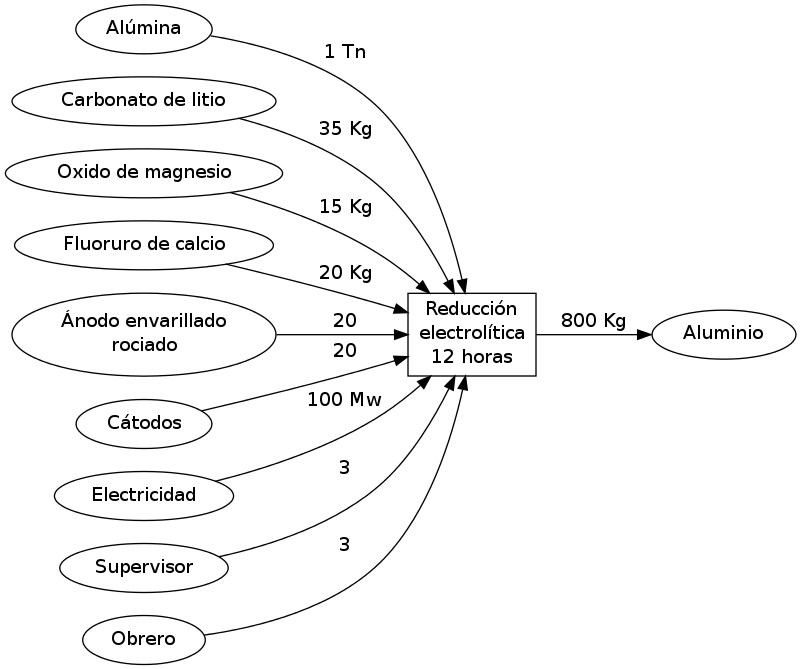
\includegraphics[scale=0.3]{alumina.png}
    \end{center}
    \caption{Ejemplo de representación pictórica de un  proceso
    hipotético de producción de aluminio} 
    \label{proceso:fig}
    \label{aluminio:fig}
   \end{figure}

   En el grafo los procesos se distinguen mediante nodos rectangulares,
   mientras que los bienes mediante nodos elípticos. Los bienes situados
   a la izquierda del proceso se califican de \mbox{``bienes de
   entrada''} o ``insumos'' mientras que los de la derecha son
   \mbox{``bienes de salida''}. Aunque en la vida real un proceso podría
   tener más de un bien de salida, por simplicidad en este trabajo
   asumimos que un proceso produce un solo bien.

   Los arcos emanantes de los bienes de entrada son llamados de
   \mbox{``entrada''}; análogamente, los arcos emanantes del proceso son
   llamados de \mbox{``salida''}.

   Tanto el proceso como sus arcos relacionan datos que contribuyen al
   cálculo y determinación de información. Básicamente, a cada arco de un
   proceso se le atribuye la cantidad del insumo requerido si es un
   arco de entrada, o la cantidad de bien que se produce si es un arco de
   salida. Si los arcos de entrada se relacionan con costes de
   adquisición, entonces se puede calcular un coste de producción.

   En el ejemplo de la figura~\ref{proceso:fig} se muestra que el proceso
   ``Reducción~electrolítica'' produce 800 Kg de aluminio mediante 1 Tn
   de alúmina, 35 Kg de carbonato de litio, 15 Kg de óxido de magnesio,
   20 Kg de fluoruro de calcio, 20 ánodos, 20 cátodos, 100 Mw de potencia
   eléctrica, tres supervisores y tres obreros.

   A un proceso se le vinculan algunos tiempos: tiempo de operación, que
   es la duración que el proceso consume para la producción de sus
   bienes de salida y el tiempo de construcción, que es el tiempo que se
   emplearía para construir una instancia física del proceso. 

   No hay restricciones sobre las cantidades de procesos y sus
   especificaciones. Un bien dado puede producirse de muchísimas maneras,
   ergo mediante muchos tipos de procesos. Distintos procesos pueden
   producir exactamente el mismo bien, inclusive pueden ser idénticos,
   tanto en la composición de sus insumos como en las cantidades de
   insumos y del bien producido.

   \subsubsection{Productor}\label{productor:sec}



   \subsubsection{Red productiva}

   \subsection{Componentes del modelo}

  \subsection{Factibilidad de modelo}

   \subsubsection{Representatividad}

   \subsubsection{Vigencia}

   \subsubsection{El impacto del  mercado en las relaciones
   productivas}\label{mercado:sec} 

   \subsubsection{Facilidad de obtención}

   \subsubsection{Invariabilidad de los arcos productivos}

   \subsubsection{Coste versus precio}

 \section{Aplicación de grafos a estudios económicos}

  \subsection{Vistas de una red productiva}

   \subsubsection{Mapa de procesos}

   \subsubsection{Mapa de producción} \label{mapa-produccion:fig}

   \subsubsection{Mapa potencial de producción}

   \subsubsection{Mapa de propiedad de la producción}

   \subsubsection{Grafo de dependencias de un bien}

   \subsubsection{Cortes de red}

  \subsection{Fiscalización e inferencia tecnológica}
  \label{fiscal:sec}

  \subsection{Observación de la propiedad}
  \label{monopolio:sec}
  \label{monopolios:sec}


  \subsection{Satisfacción de demanda y plan de producción}
  \label{demanda:sec}

   \subsubsection{Satisfacción de demanda}

   \subsubsection{Cálculo de plan de producción de una demanda}


   \section{Aplicación a casos reales}

   


 

 \end{document}

